\documentclass[11pt]{article}

% ======================
% Packages
% ======================
\usepackage[utf8]{inputenc}
\usepackage[T1]{fontenc}
\usepackage{lmodern}
\usepackage{amsmath,amssymb,amsthm}
\usepackage{geometry}
\usepackage{listings}
\usepackage{xcolor}
\usepackage{graphicx}
\usepackage{algorithm}
\usepackage{algpseudocode}
\usepackage{hyperref}
\usepackage{enumitem}
\usepackage{tikz}
\usepackage{array}
\usepackage{booktabs}
\usepackage{caption}

\usetikzlibrary{arrows.meta,positioning}

% ======================
% Page Layout
% ======================
\geometry{a4paper, margin=1in}
\setlength{\parindent}{0pt}
\setlength{\parskip}{1em}

% ======================
% Colors & Code Styling
% ======================
\definecolor{codegreen}{rgb}{0,0.6,0}
\definecolor{codegray}{rgb}{0.5,0.5,0.5}
\definecolor{codepurple}{rgb}{0.58,0,0.82}
\definecolor{backcolour}{rgb}{0.95,0.95,0.92}

\lstdefinestyle{mystyle}{
    backgroundcolor=\color{backcolour},
    commentstyle=\color{codegreen},
    keywordstyle=\color{magenta},
    numberstyle=\tiny\color{codegray},
    stringstyle=\color{codepurple},
    basicstyle=\ttfamily\small,
    breakatwhitespace=false,
    breaklines=true,
    captionpos=b,
    keepspaces=true,
    numbers=left,
    numbersep=5pt,
    showspaces=false,
    showstringspaces=false,
    showtabs=false,
    tabsize=2
}

\lstset{style=mystyle}

% ======================
% Theorem-like Environments
% ======================
\newtheorem{problem}{Problem}
\newtheorem{subproblem}{Subproblem}[problem]
\newtheorem{solution}{Solution}[problem]

% ======================
% Title Info
% ======================
\title{\textbf{Fundamental Algorithm Techniques} \\ Problem Set \#8}
\date{\textcolor{red}{Review on April 9}}

% ======================
% Document
% ======================
\begin{document}

\maketitle

\begin{problem}[Graph Colouring, 5 pts]

\begin{enumerate}
    \item Describe Sudoku as a graph colouring problem and explain the boundary conditions.
\end{enumerate}

\end{problem}

\begin{problem}[Bellman--Ford Algorithm, 5 pts]

\begin{center}
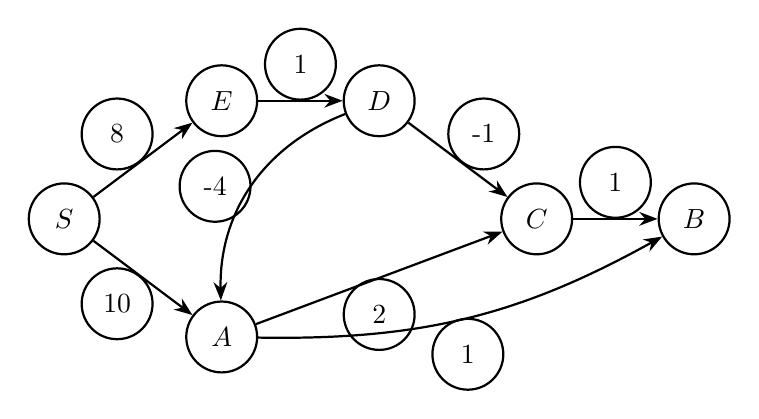
\begin{tikzpicture}[
    >=Stealth,
    every node/.style={circle, draw, minimum size=9mm},
    every path/.style={->, thick}
]

\node (S) at (0,0) {$S$};
\node (E) at (2,1.5) {$E$};
\node (A) at (2,-1.5) {$A$};
\node (D) at (4,1.5) {$D$};
\node (C) at (6,0) {$C$};
\node (B) at (8,0) {$B$};

\draw (S) -- node[above left] {8} (E);
\draw (S) -- node[below left] {10} (A);
\draw (E) -- node[above] {1} (D);
\draw (D) -- node[above right] {-1} (C);
\draw (D) to[bend right=35] node[left] {-4} (A);
\draw (A) -- node[below] {2} (C);
\draw (A) to[bend right=15] node[below] {1} (B);
\draw (C) -- node[above] {1} (B);

\end{tikzpicture}
\end{center}




Consider the directed weighted graph above with edges:
\[
S \to E = 8,\quad
S \to A = 10,\quad
E \to D = 1,\quad
D \to C = -1,
\]
\[
D \to A = -4,\quad
A \to C = 2,\quad
A \to B = 1,\quad
C \to B = 1.
\]

\begin{enumerate}
    \item Run the Bellman--Ford algorithm starting from source vertex $S$.
    \item Show the distance estimate after each iteration.
    \item Give the final shortest-path distance from $S$ to every other vertex.
    \item Explain why Dijkstra's algorithm cannot be run correctly on the above graph.
    \item State whether the graph contains a negative cycle.
\end{enumerate}

\end{problem}

\end{document}
